%%%%%%%%%%%%%%%%%%%%%%%%%%%%%%%%%%%%%%%%%%%%%%%%%%%%%%%%%%%%%%%%%
%%  To create image run: (for Windows use imgconvert)
%%
%%  convert -verbose -delay 50 -loop 0 -density 300 -resize 640x480 src/<NAME>.pdf images/<NAME>.gif
%%
%%%%%%%%%%%%%%%%%%%%%%%%%%%%%%%%%%%%%%%%%%%%%%%%%%%%%%%%%%%%%%%%
\documentclass[beamer,tikz,preview]{standalone}
%\documentclass{beamer}

%\setbeamertemplate{navigation symbols}{}
\usepackage{tikz}
\usepackage{color}

\tikzset{pics/.cd,
cube/.style args={#1/#2/#3/#4}{code={
\coordinate (O) at (0,0,0);
\coordinate (A) at (0,#2,0);
\coordinate (B) at (0,#2,#3);
\coordinate (C) at (0,0,#3);
\coordinate (D) at (#1,0,0);
\coordinate (E) at (#1,#2,0);
\coordinate (F) at (#1,#2,#3);
\coordinate (G) at (#1,0,#3);
\draw[black,fill=black!80] (O) -- (C) -- (G) -- (D) -- cycle;
\draw[black,fill=black!30] (O) -- (A) -- (E) -- (D) -- cycle;
\draw[black,fill=black!10] (O) -- (A) -- (B) -- (C) -- cycle;
\draw[black,fill=black!20,opacity=0.8] (D) -- (E) -- (F) -- (G) -- cycle;
\draw[black,fill=black!20,opacity=0.6] (C) -- (B) -- (F) -- (G) -- cycle;
\draw[black,fill=black!20,opacity=0.8] (A) -- (B) -- (F) -- (E) -- cycle;
\node at (0.5*#1,0.5*#2,0.5*#3) {#4};
}}}
\tikzset{pics/.cd,
lwing/.style args={#1/#2/#3/#4}{code={
\coordinate (O) at ( 0, 0, 0);
\coordinate (A) at ( 0, 0,#3);
\coordinate (B) at ( 0,#2,#3);
\coordinate (C) at ( 0,#2, 0);
\draw[black,fill=red!20] (O) -- (A) -- (B) -- (C) -- cycle;
\node at (0,0.5*#2,0.5*#3) {#4};
}}}
\tikzset{pics/.cd,
mwing/.style args={#1/#2/#3/#4}{code={
\coordinate (O) at ( 0, 0, 0);
\coordinate (A) at (#1, 0, 0);
\coordinate (B) at (#1,#2, 0);
\coordinate (C) at ( 0,#2, 0);
\draw[black,fill=green!20] (O) -- (A) -- (B) -- (C) -- cycle;
\node at (0.5*#1,0.5*#2,0) {#4};
}}}
\tikzset{pics/.cd,
rwing/.style args={#1/#2/#3/#4}{code={
\coordinate (O) at ( 0, 0, 0);
\coordinate (A) at (#1, 0, 0);
\coordinate (B) at (#1, 0,#3);
\coordinate (C) at ( 0, 0,#3);
\draw[black,fill=blue!20] (O) -- (A) -- (B) -- (C) -- cycle;
\node at (0.5*#1,0,0.5*#3) {#4};
}}}

\begin{document}
\begin{frame}
%\begin{center}
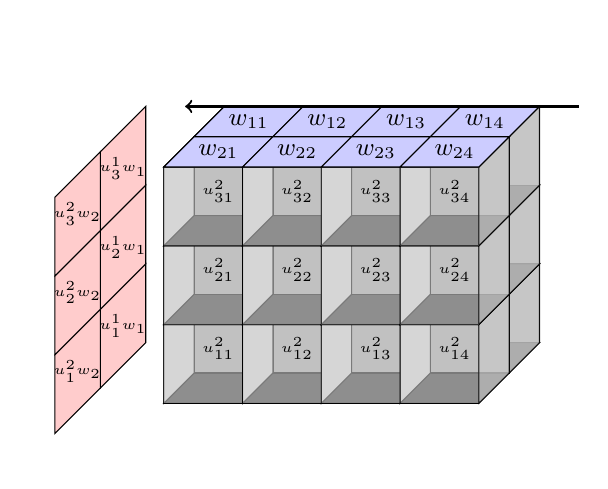
\begin{tikzpicture}
    \foreach \y/\valy in {0/1,1/2,2/3} {
        \foreach \x in {1,...,4} {
            \foreach \z/\valz in {0/1,1/2} { 
                \pic at (\x,\y,\z) {cube={1/1/1/{\tiny $u^{\valz}_{\valy\x}$}}};
                
            };
        }
    }
    \foreach \x in {1,...,4}{
        \foreach \z/\valz in {0/1,1/2} 
            {\pic at (\x,3,\z) {rwing={1/1/1/{\small $w_{\valz\x}$}}};}
    }
    \draw[thick,->] (5.5,3) -- (0.5,3);
    %\pause    
    \foreach \n in {4,3,2,1} {
        \pause
        \fill[color=white] (-1.5,-1.5) rectangle (5.5,4);
        \draw[thick,->] (\n+0.5,3) -- (0.5,3);
        \foreach \x in {1,...,\n} {    
            \foreach \y/\valy in {0/1,1/2,2/3} {
                \foreach \z/\valz in {0/1,1/2} { 
                    \pic at (\x,\y,\z) {
                        cube={1/1/1/{\tiny $u^{\valz}_{\valy\x}w_{\valz\x}$}}
                    };                
                };
            }
        }
        \foreach \y/\valy in {0/1,1/2,2/3} {
            \foreach \z/\valz in {0/1,1/2} { 
                 \pic at (\n,\y,\z) {
                    cube={1/1/1/{\tiny $\sum_i u^{\valz}_{\valy i} w_{\valz i}$}}
                };
            }
        }
    }
    \pause
    \fill[color=white] (-1.5,-1.5) rectangle (5.5,4);
    \foreach \y/\valy in {0/1,1/2,2/3} {
        \foreach \z/\valz in {0/1,1.5/2} { 
             \pic at (0,\y,\z) {
                lwing={1/1/1.5/{\tiny $u^{\valz}_{\valy} w_{\valz}$}}
            };
        }
    }
    \pause
    \foreach \y/\valy in {0/1,1/2,2/3} {
        \foreach \x in {1,...,4} {
            \foreach \z/\valz in {0/1,1/2} { 
                \pic at (\x,\y,\z) {cube={1/1/1/{\tiny $u^{\valz}_{\valy\x}$}}};
                
            };
        }
    }
    \foreach \x in {1,...,4}{
        \foreach \z/\valz in {0/1,1/2} 
            {\pic at (\x,3,\z) {rwing={1/1/1/{\small $w_{\valz\x}$}}};}
    }
    \draw[thick,->] (5.5,3) -- (0.5,3);
\end{tikzpicture}
%\end{center}
\end{frame}

\end{document}